% -*- root: ../../DAT2-A423_Project_Report.tex -*-
\section{Interfaces}
\section{Implementation of a JPEG image}
Looking back to section \ref{sec:designJPEG} we can start implementing this into our steganography program \textit{Stegasaurus}.
We can also refer to figure \ref{fig:JPEGprocess} for the steps the encoder must take.

There are multiple constructors for the \lstinline|JPEGImage| class, as a user can choose to specify custom quantization- or Huffman tables, or simply use the default table which both the \lstinline|QuantizationTable|- and \lstinline|HuffmanTable| classes provide, by not providing any tables in the constructor.
The default tables in the respective classes are both found in the JPEG specification \citep[Annex k]{JPEGStandard}.

The \lstinline|void Encode(byte[])| is where the actual JPEG encoding takes place.
The method can be seen in listing \ref{JPEGEncode}.
The most significant part of the JPEG file is obviously the scan data, but before that can be written to the file, we have to encode most of the headers first.
We do that by calling \lstinline|void _writeHeaders()|.
All information needed in these headers are already known, as both the bitmap image and tables provided in the constructor.

\begin{lstlisting}[firstnumber=136,label=JPEGEncode, caption={\lstinline|JPEGImage.Encode| method \textbf{File: }JPEGImage.cs}]
public void Encode(byte[] message) {
    //Instantiate a JpegWriter, which has an internal list of bytes 
    //and the logic required to write those to a file
    _jw = new JpegWriter();

    if (message.Length > 16884) {
        throw new ArgumentException("Message cannot be longer than 16884 bytes!");
    }
    _breakDownMessage(message);

    _writeHeaders();
    _writeScanData();
    _writeEndOfImage();
}
\end{lstlisting}

From here on, we need to perform all of the regular steps from JPEG encoding up until just before the Huffman encoding.
We start out with splitting the image into Y, Cb and Cr channels instead of the \lstinline|Bitmap|'s RGB channels, and then in the method \lstinline|void _encodeAndQuantizeValues(sbyte[][,], int, int)| we have the loop which can be seen in listing \ref{JPEGEncodeAndQuantize}.
While these nested loops may seem very computationally heavy, what it actually does is that it loops through the three channels of every pixel in the 16x16 MCU's.
So while we have five nested for loops, we run through every pixel 3 times.
After every 16x16 MCU has been filled with values, the MCU must be encoded.
As the name Minimum Encoded Unit implies, we can encode one MCU without depending on the other.
That means that after we fill one MCU, we can encode that directly. We do that by invoking the method \lstinline|void _encodeBlocks(float[][,])|.

\begin{lstlisting}[firstnumber=525, label=JPEGEncodeAndQuantize, caption={Shows how the image is divided into MCUs \textbf{File: }JPEGImage.cs}]
for (int MCUY = 0; MCUY < imageHeight; MCUY += 16) {
    for (int MCUX = 0; MCUX < imageWidth; MCUX += 16) {
        for (int i = 0; i < 3; i++) {
            for (int x = 0; x < 16; x++) {
                for (int y = 0; y < 16; y++) {
                    channels[i][x, y] = YCbCrChannels[i][MCUX + x, MCUY + y];
                }
            }
        }
        _encodeBlocks(channels);
    }
}
\end{lstlisting}

In this method, we split the MCU into 8x8 blocks.
As we have a fixed sampling of 4:2:0 that means that we split the Y channel into four 8x8 blocks and effectively save all information about the luminance channel, the Cr and Cb channels, we down-sample from a 16x16 block to a 8x8 blocks.
As we implemented this, we had two ways of doing so.
One way of doing it, is taking every 4th value in the block as seen on figure \ref{fig:downsampling4th}, and the other way of doing it, is taking an average of each 2x2 block in the 16x16 MCU as seen on figure \ref{fig:downsamplingAverage}.

\begin{figure}
    \centering
    \begin{subfigure}[b]{0.3\textwidth}
        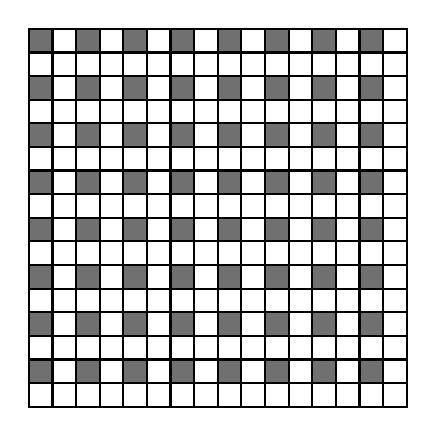
\begin{tikzpicture}
    [%%%%%%%%%%%%%%%%%%%%%%%%%%%%%%
        box/.style={rectangle,draw=black,thick, minimum size=0.3cm},scale=0.3
    ]%%%%%%%%%%%%%%%%%%%%%%%%%%%%%%

\foreach \x in {0,1,...,15}{
    \foreach \y in {0,1,...,15}
        \node[box] at (\x,\y){};
}

\foreach \x in {0,2,4,6,8,10,12,14}{
    \foreach \y in {1,3,5,7,9,11,13,15}
        \pgfmathparse{44}
        \edef\tmp{\pgfmathresult}
        \node[box,fill=white!\tmp!black] at (\x,\y){};
} 

\end{tikzpicture}
        \caption{Downsampling by choosing only every 4th value}
        \label{fig:downsampling4th}
    \end{subfigure}
    \qquad %add desired spacing between images, e.g.~, \quad, \qquad, \hfill etc. 
      %(or a blank line to force the subfigure onto a new line)
    \begin{subfigure}[b]{0.3\textwidth}
        \begin{tikzpicture}
    [%%%%%%%%%%%%%%%%%%%%%%%%%%%%%%
        box/.style={rectangle,draw=black,thick, minimum size=0.6cm},scale=0.6
    ]%%%%%%%%%%%%%%%%%%%%%%%%%%%%%%

\foreach \x in {0,1,...,7}{
    \foreach \y in {0,1,...,7}
        \node[box] at (\x,\y){};
}
\foreach \x in {0,1,...,7}{
    \foreach \y in {0,1,...,7}
        \pgfmathparse{\intcalcMod{\x}{2} * 22 + \intcalcMod{\y}{2} * 22 + 22}
        \edef\tmp{\pgfmathresult}
        \node[box,fill=white!\tmp!black] at (\x,\y){};
}

\end{tikzpicture}
        \caption{Downsampling by taking an average of every four values}
        \label{fig:downsamplingAverage}
    \end{subfigure}
    \caption{Different methods for downsampling of 16x16 MCU to an 8x8 block}\label{fig:downsampling}
\end{figure}


In our implementation we chose to use the average.
While it does take some more calculations, we do get better image quality.
The problem with using just one value for every 2x2 block, is that if the image contains sharp edges, those lines will become distorted.
If using the average instead, the lines will, at most, become a bit blurry.

After the down-sampling process, only the DCT and Quantization processes are left before we can start embedding the message.
On each 8x8 block we perform DCT as seen in listing \ref{JPEGEncodeDCT}.
The DCT formula was described in section \ref{sec:jpegStudy}, but one thing we realised about the formula was, that we could calculate the cosines only once, and use these instead of repeatedly calculating the trigonometric function, therefore we calculate these results before even beginning the DCT process, and then just reuse the results in the DCT method.
 

\begin{lstlisting}[firstnumber=603,label=JPEGEncodeDCT, caption={Multidimensional DCT on 8x8 block \textbf{File: }JPEGImage.cs}]
private static float[,] _discreteCosineTransform(float[,] block8) {
    float[,] cosineValues = new float[8, 8];

    for (int i = 0; i < 8; i++) {
        for (int j = 0; j < 8; j++) {
            float tempSum = 0.0f;
            float cCoefficient = _c(i, j);
            for (int x = 0; x < 8; x++) {
                for (int y = 0; y < 8; y++) {
                    tempSum += cCoefficient * block8[x, y] * CosinesCoefficients[x, i] * CosinesCoefficients[y, j];
                }
            }
            cosineValues[i, j] = tempSum;
        }
    }
    return cosineValues;
}
\end{lstlisting}

\FloatBarrier

After calculating the DCT coefficients, it is simply a matter of dividing each entry in the 8x8 block with the corresponding value in the quantization table.

We wanted our JPEG encoder to be able to have a quality setting, so that the user of the class can choose wether they want to focus on image size or image quality. To lower the filesize, and also the quality we must divide by larger values in the quantisation step. The way we do this, is that we scale the quantization table based on an integer between 0 and 100 (the quality setting).

We use the function $f(q) = \frac{100-x}{53}+0.125$ to convert from a quality to a factor we can multiply the entries in the quantization table with. There is no standard function for choosing multiplication factors, so we just chose a function that will scale nicely between the numbers 0 and 100. On figure \ref{fig:plotQuality} a plot of the function is seen.

After the scaling process, we divide each entry in the DC coefficients by the corresponding entry in the quantization table. The results of this process are saved to the private field \lstinline|_quantizedValues|.


\begin{figure}
    \centering
    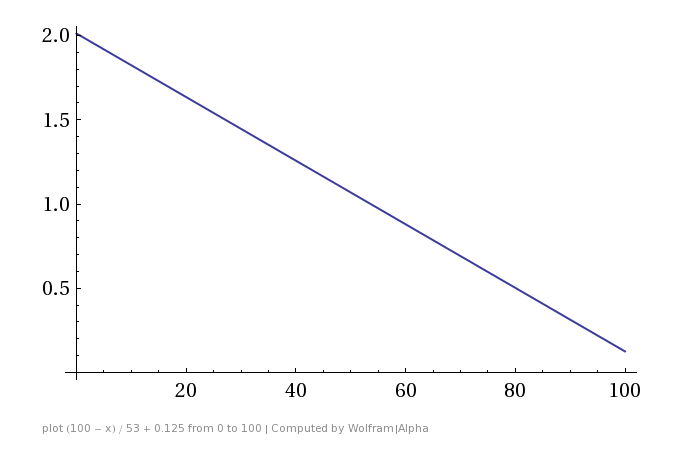
\includegraphics[width=0.5\textwidth]{figures/plotQuality.png}
    \label{fig:plotQuality}
    \caption{Plot of $f(q) = \frac{100-x}{53}+0.125$ that shows how the quality of the jpeg image impacts the quantization tables}
\end{figure}

So now we are ready to perform the actual encoding of the data, before saving the image data to a file.
We use procedure \ref{algJPEG} to find the valid entries from our newly filled \lstinline|_quantizedValues|.
The first 16 values from our valid entries, we add as vertices to the graph, with a modulo of 4 as the length and modulo value will always be encoded with modulo 4 so that it can be decoded.
Then we keep on adding vertices, until we are certain that we have enough vertices to embed all the data in the \lstinline|byte[]|.
After adding the vertices, we use the private method \lstinline|void _addEdge(bool, bool, Vertex, Vertex, int, Graph)| to determine whether an edge between the two specified vertices would result in a perfect pair.
If the edge would result in a perfect pair, the edge is added to the graph.

We run this method 4 times for every distinctive pair of vertices in the graph, for each of the possible switches shown earlier in figure \ref{fig:graphSwitches}.
In procedure \ref{algJPEGEncode} we would loop every vertex, for each vertex.
If we had the vertices $\{a,b,c,d\}$ we would get the pairs $\{(a,b),(a,c),(a,d)(b,a),(b,c),(b,d),(c,a),(c,b),(c,d),(d,a),(d,b),(d,c)\}$.
To find all possible switches, there is no need to check both $(a,b)$ and $(b,a)$, as those two vertices would have the same switches.
In fact, we only need to check the switches $\{(a,b),(a,c),(a,d),(b,c),(b,d),(c,d)\}$, which is half of the original pairs.
We implemented this as seen in listing \ref{implementationPairs}.
The inner loop starts at the vertex following the current vertex in the outer loop.
This way, we do not find the reversed counterparts of already found pairs.
This particular piece is still $\mathcal{O}(n^2)$, but instead of checking $n(n-1)=n^2-n$ pairs, we only need to check $(n\cdot\frac{n}{2})=\frac{n^2}{2}$ where $n$ is the number of vertices. 


\begin{lstlisting}[firstnumber=655,label=implementationPairs,caption={Checks all edges between distincive pairs of vertices \textbf{File: }JPEGImage.cs}]
Parallel.For(0, length, i => {
    for (int j = i + 1; j < length; j++) {
        _addEdge(true, true, toBeChanged[i], toBeChanged[j], threshold, graph);
        _addEdge(true, false, toBeChanged[i], toBeChanged[j], threshold, graph);
        _addEdge(false, true, toBeChanged[i], toBeChanged[j], threshold, graph);
        _addEdge(false, false, toBeChanged[i], toBeChanged[j], threshold, graph);
    }
});
\end{lstlisting}

After adding the edges, we need to determine what edges to keep, where each edge describes a switch between two vertices.
We do that by sorting our edges by weight and then choose the edge with the lowest weight. We then remove all other edges connected to the two vertices connected by the chosen edge, and then repeat the process.
All of this is implemented as seen in listing \ref{graphDoSwitches}.

\begin{lstlisting}[firstnumber=14,label=graphDoSwitches, caption={Implementation of greedy algorithm for choosing switches \textbf{File: }JPEGImage.cs}]
public List<Edge> GetSwitches() {
    Edges.Sort();
    List<Edge> chosenEdges = new List<Edge>();
    while (Edges.Any()) {
        chosenEdges.Add(Edges[0]);
        _removeEdge(Edges, Edges[0]);
    }
    return chosenEdges;
}

private static void _removeEdge(List<Edge> list, Edge e) {
    list.RemoveAll(x => x.VStart == e.VStart || x.VStart == e.VEnd || x.VEnd == e.VStart || x.VEnd == e.VEnd);

\end{lstlisting}

After running the \lstinline|List<Edge> GetSwitches| method on the graph, it was simply a matter of switching the values in the vertices appointed by the chosen edges, and then running through all of the vertices in the graph, and for every vertex not containing the right message, forcibly change the sample values so that the right message is contained.


The only thing needed before saving the image to the file, is the Huffman encoding.
The process of doing this is relatively trivial.
We start out by encoding the DC as seen in listing \ref{DCencoding}. We do that by first finding the difference from the last DC entry (in the current MCU), then finding the Huffman code from the DC Huffman table, before saving the bits to the image.

\begin{lstlisting}[label=DCencoding,caption={Encoding DC coefficient into the image \textbf{File: }JPEGImage.cs}]
short diff = (short)(block8[0, 0] - _lastDc[DCIndex]);
_lastDc[DCIndex] += diff;

if (diff != 0) {
    byte category = _bitCost(diff);
    HuffmanElement huffmanCode = huffmanDC.GetElementFromRunSize(0, category);
    _ushortToBits(bits, huffmanCode.CodeWord, huffmanCode.Length);

    _ushortToBits(bits, _numberEncoder(diff), category);
} else {
    HuffmanElement EOB = huffmanDC.GetElementFromRunSize(0x00, 0x00);
    _ushortToBits(bits, EOB.CodeWord, EOB.Length);
}
\end{lstlisting}

Now the next part of the Huffman encoding is simply to run through the 63 AC values in zigzag.
If we find a zero, we count that, but otherwise keep on going as that zero must be encoded as EOB, ZRL or as part of the next non-zero value.
If we have more than 16 zeroes before the next non-zero value we encode the ZRL, and if the rest of the block consists of only zeroes, we encode the EOB. This can all be seen in listing \ref{ACencoding}

\begin{lstlisting}[label=ACencoding,caption={Encoding AC coefficients into the image \textbf{File: }JPEGImage.cs}]
int zeroesCounter = 0;
for (int i = 1; i < 64; i++) {
    int x = QuantizationTable.RoadPoints[i, 0], y = QuantizationTable.RoadPoints[i, 1];
    if (block8[x, y] == 0) {
        zeroesCounter++;
        continue;
    }
    while (zeroesCounter >= 16) {
        HuffmanElement ZRL = huffmanAC.GetElementFromRunSize(0x0F, 0x00);
        _ushortToBits(bits, ZRL.CodeWord, ZRL.Length);
        zeroesCounter -= 16;
    }

    byte cost = _bitCost(Math.Abs(block8[x, y]));
    HuffmanElement codeElement = huffmanAC.GetElementFromRunSize((byte)zeroesCounter, cost);
    zeroesCounter = 0;
    _ushortToBits(bits, codeElement.CodeWord, codeElement.Length);

    _ushortToBits(bits, _numberEncoder(block8[x, y]), cost);
}

if (zeroesCounter != 0) { //EOB
    HuffmanElement EOB = huffmanAC.GetElementFromRunSize(0x00, 0x00);
    _ushortToBits(bits, EOB.CodeWord, EOB.Length);
}
\end{lstlisting}

After the Huffman encoding, it is simply a matter of adding the EOI marker to the end of the image, and saving the bytes to a file. 

\subsection{Working with bits}
While working with JPEG images we found that bit-patterns and bit-wise operations often occur.
Due to hardware limitations, a single bit in the memory cannot be changed individually, and we can only address the individual bytes.
There are now two ways that we can go about this:
Either we use bytes to represent bits, and effectively waste 7 bits of memory for each bit, or we use the class \lstinline|BitArray| from the \lstinline|System.Collections| library.
What this class does, is that it handles the packing of the bits into bytes, and makes you able to address the individual bits.

The \lstinline|BitArray| seemed like the way to go, and we implemented a class \lstinline|BitList| which implemented List-like features like \lstinline|Add| and \lstinline|Insert| while using the \lstinline|BitArray| to store our data.
The implementation can be seen in appendix \ref{app:C}. 

The \lstinline|BitArray| offers the functionality of modifying the length of the array, so that more values can be added.
This means that every time the \lstinline|BitList| runs out of space in the underlying \lstinline|BitArray|, we simply multiply the length of the array by 2, so that more values can be added.
This makes appending to the array relatively fast, since we have enough room to add more values most of the time.
Inserting values in the middle of the array, however, proved to be much more difficult.

When inserting a value into the array, all values after the value to be inserted have to be shifted, so that room is made from the new value.
In an example 512x512 image, we have over 750,000 bits to save, and if we were to insert a bit in the beginning of the array, we would have to move 750,000 elements in the array.
All in all a very computationally expensive operation.

So while the \lstinline|BitArray| seemed promising in theory, saving us a lot of memory, the need of inserting bits into the middle of the array makes using the \lstinline|BitArray| not feasible.
What we would need to solve this problem is to eliminate the need to shift a large part of the array. 
One way of solving this problem is to make a data type which combines the functionality of the \lstinline|BitArray| with a linked list. 
By splitting up the large \lstinline|BitArray| into smaller linked arrays we could shift the values in the smaller arrays. 
We would have a slightly longer access time, but have a much faster insertion time. 
Another way to solve the problem, and what we ended up doing, was to eliminate the need of inserting the values. 
We realised that the only time we need to insert values into the \lstinline|BitList| was when there were 8 consecutive ones in the scan data. 
So what we did was to create the method \lstinline|CheckedAdd| which we would use while writing scan data to the list. 
This method would then keep track of the last inserted values, and insert the zeroes on-the-fly instead of after the whole process. 
The method \lstinline|CheckedAdd| can also be seen in appendix \ref{app:C}.